\documentclass[11pt, oneside]{article} 
\usepackage{geometry}
\geometry{letterpaper} 
\usepackage{graphicx}
	
\usepackage{amssymb}
\usepackage{amsmath}
\usepackage{parskip}
\usepackage{color}
\usepackage{hyperref}

\graphicspath{{/Users/telliott_admin/Dropbox/Tex/png/}}
% \begin{center} 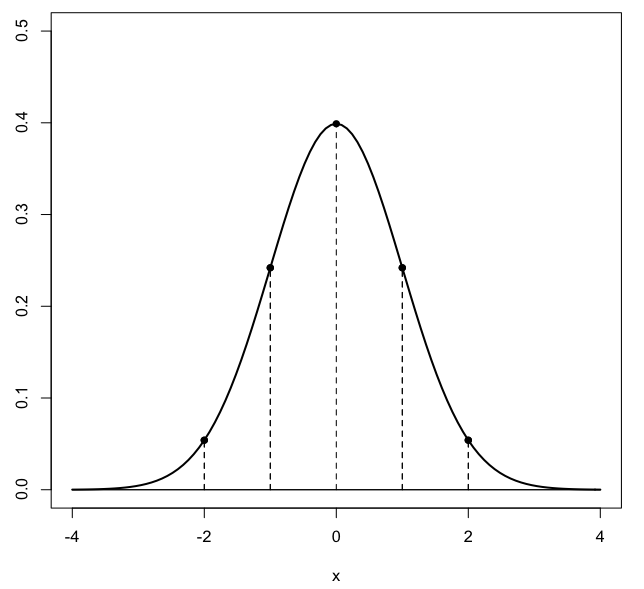
\includegraphics [scale=0.4] {gauss3.png} \end{center}

\title{Introduction}
\date{}

\begin{document}
\maketitle
\Large
This was supposed to be a short book, an exploration of problems like the volume of the cone and sphere, or even just the area of a circle, with some simple physics thrown in.  These questions contain within them the heart of calculus:  infinities both large and small.  I imagine myself looking over Archimedes' shoulder as he explains it to me.

I wrote many of the early chapters originally as short explanations for my son Sean as he studied calculus in high school.  It bothers me that so often the good stuff gets left out --- the ideas which make you go ... wow.  Now, years later, I still find a lot of pleasure in trying to understand what Kepler and Newton did.  It took a genius to figure it out the first time, but it is within anyone's grasp to appreciate what they found.

Then I thought, why not include other favorite problems like the area of the ellipse, the "headlight" problem for the parabola, or the reflective property of the ellipse, and the length and area under the cycloid curve (the "light on a bicycle wheel"). These are problems where calculus easily produces answers that can be checked by more elaborate geometric arguments.  So here we are, with a somewhat longer book.

In the introduction to his book \emph{Calculus}, Morris Kline says
\begin{quote}Anyone who adds to the plethora of introductory calculus texts owes an explanation, if not an apology, to the mathematical community.\end{quote}

I think of this book as a form of ultralight backpacking.  We shed weight so as to ascend peaks rapidly, skimming the best of calculus --- focusing on geometry and physics, and slinging differentials with abandon.  Epsilon appears mainly as the physics constant $\epsilon_o$.  Starting with an intuitive notion of adding up many small pieces, we put integrals to work early solving problems.

Going fast allows time to get a view of sophisticated topics, among others, line integrals for work and flux, Newton's proof that a spherical mass acts as a point mass, and integration of a parametrized surface like the torus.  Not to mention Kepler's Laws, and a derivation of the Gaussian distribution from first principles.

We do not disdain proof.  On the contrary, \emph{interesting} proofs are much to be admired.  We prove the Pythagorean Theorem, and the quotient rule for derivatives, as well as Green's Theorem.  There is a fun chapter on induction.

My favorite authors are Morris Kline, Richard Hamming, and Gil Strang.  Sylvanus Thompson's simple book is my favorite first text, and it's even a Project Gutenberg project:

\url{https://www.gutenberg.org/files/33283/33283-pdf.pdf}

Having said what I like, briefly, here are some things I don't like.

The rigorous approach to calculus pioneered by Cauchy in the 1820's and exported to American schools by Richard Courant in the 1940's is a bad idea.  We must motivate rigorous proof by demonstrating utility first.  As Ian Stewart says, "proofs come \emph{after} understanding."  Courant's method is the way to teach the subject the second  \emph{or third} time through.

Thompson:

\begin{quote}
You don't forbid the use of a watch to every person who does not know how to make one. You don't object to the musician playing on a violin that he has not himself constructed. You don't teach the rules of syntax to children until they have already become fluent in the use of speech. It would be equally absurd to require general rigid demonstrations to be expounded to beginners in the calculus.\end{quote}

A second thing I dislike is calculus problems that are gratuitously arithmetic.  Calculus comes from bright ideas, not complicated ones;  if the computation is difficult, it's usually \emph{not} a good problem.  Also, a good problem often is one with a physical or practical foundation.  Having said that, if a course could integrate elementary programming with calculus, I would be very happy.

I express my sincere thanks to the authors of my favorite books, which are listed in the references and mentioned at various places in the text.  Almost everything in here was appropriated from them, and styled to my taste.  I offer my profound thanks also to Eugene Colosimo, S.J.  He was, for me, the best of a bunch of very special teachers.

If I stole your figure off the internet, I'm sorry.  I intended to redraw it but have not yet found the time.  

We start with my favorite mathematician, Archimedes.

[ Update:  Over time, I have added quite a bit of geometry.  At this point, the title might as well be \emph{Best of Calculus and Geometry}. ]

---

You can find the book on github here:

\url{https://github.com/telliott99/Tex/tree/master/calculus_book}

\end{document}